\def\circledarrow#1#2#3{ % #1 Style, #2 Center, #3 Radius
    \draw[#1,latex-latex] (#2) +(50:#3) arc(50:-230:#3);
}
\begin{figure}[h]
    \centering
    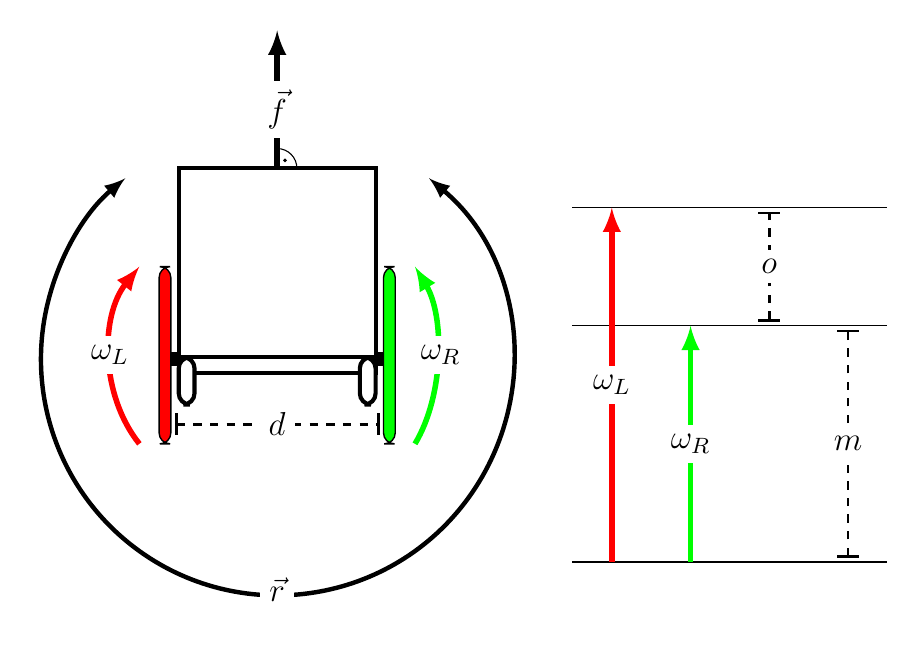
\begin{tikzpicture}[scale=0.5]
        \draw[line width=1, fill=black] (-2.9,0) rectangle (2.9,0.3); %radachse
        \draw[line width=1.5, fill=white] (-2.5,0) rectangle (2.5,5); %sitz
        \draw[line width=1.5, fill=white] (-2.5,-0.2) rectangle (2.5,0.2); %lehne
        \draw[line width=1.5, fill=white, rounded corners] (-2.5,0.2) rectangle (-2.1,-1); %griff links
        \draw[line width=1.5, fill=white, rounded corners] (2.1,0.2) rectangle (2.5,-1); % griff rechts

        \draw[line width=0.5, fill=red, rounded corners] (-3,-2) rectangle (-2.7,2.5); %rad links
        \draw[line width=0.5, fill=green, rounded corners] (2.7,-2) rectangle (3,2.5); %rad rechts

        \draw (0.5,5) arc
            [
                start angle=0,
                end angle=90,
                x radius=0.5,
                y radius=0.5
            ];
        \draw[fill=black] (0.2,5.2) circle (0.03); %rechter winkel punkt

        % d
        \draw[Bar-Bar, line width=1, dashed] (-2.6,-1.5) -- (2.6,-1.5);
        \node [anchor=center, fill=white] at (0,-1.5) {\large$d$};

        % f
        \draw[-latex, line width=2] (0,5) -- (0,8.5);
        \node [anchor=center, fill=white] at (0,6.5) {\large$\vec{f}$};

        % omegaL
        \draw[-latex, line width=2, color=red] (-3.5,-2) .. controls (-4.5,-0.75) and (-4.5,1.25) .. (-3.5,2.5);
        \node [anchor=center, fill=white] at (-4.25,0.25) {\large$\omega_L$};

        % omegaR
        \draw[-latex, line width=2, color=green] (3.5,-2) .. controls (4.25,-0.75) and (4.25,1.25) .. (3.5,2.5);
        \node [anchor=center, fill=white] at (4.15,0.25) {\large$\omega_R$};

        % r
        \node (zAxis) at (0,0.15) {};
        \circledarrow{ultra thick, black}{zAxis}{6};
        \node [anchor=center, fill=white] at (0,-5.7) {\large$\vec{r}$};

        % -----------------------------------------------------

        \draw[line width=0.5] (7.5,-5) -- (15.5,-5);
        \draw[line width=0.5] (7.5,1) -- (15.5,1);
        \draw[line width=0.5] (7.5,4) -- (15.5,4);

        \draw[-latex, line width=2, color=red] (8.5,-5) -- (8.5,4);
        \node [anchor=center, fill=white] at (8.5,-0.5) {\large$\omega_L$};

        \draw[-latex, line width=2, color=green] (10.5,-5) -- (10.5,1);
        \node [anchor=center, fill=white] at (10.5,-2) {\large$\omega_R$};

        \draw[Bar-Bar, line width=1, dashed] (12.5,1.1) -- (12.5,3.9);
        \node [anchor=center, fill=white] at (12.5,2.5) {\large$o$};

        \draw[Bar-Bar, line width=1, dashed] (14.5,-4.9) -- (14.5,0.9);
        \node [anchor=center, fill=white] at (14.5,-2) {\large$m$};
    \end{tikzpicture}
    \caption{Skizze des Rollstuhls aus der Vogelperspektive mit Bewegungsvektoren}
    \label{fig:wheelchairMath}
\end{figure}